% Game as an Education Medium
\medskip
\subsection{Games Popularity Around the World}
\url{https://financesonline.com/number-of-gamers-worldwide/}
comprises of statistics, demographics, and predictions related to games and gamers 
both worldwide and by region. [Nestor Gilbert]

According to NewZoo Research (2020), there were 2.69 billion gamers in the world by the end of 2020. From the statistics, it is to be expected that the number of gamers will continue to rise, expecting to reach 2.95 billion gamers worldwide in 2022.

% Active gamers
\begin{figure}[!h]\centering
\setlength{\fboxrule}{0.2mm} % can define this in the preamble
\setlength{\fboxsep}{0.5mm}
\fbox{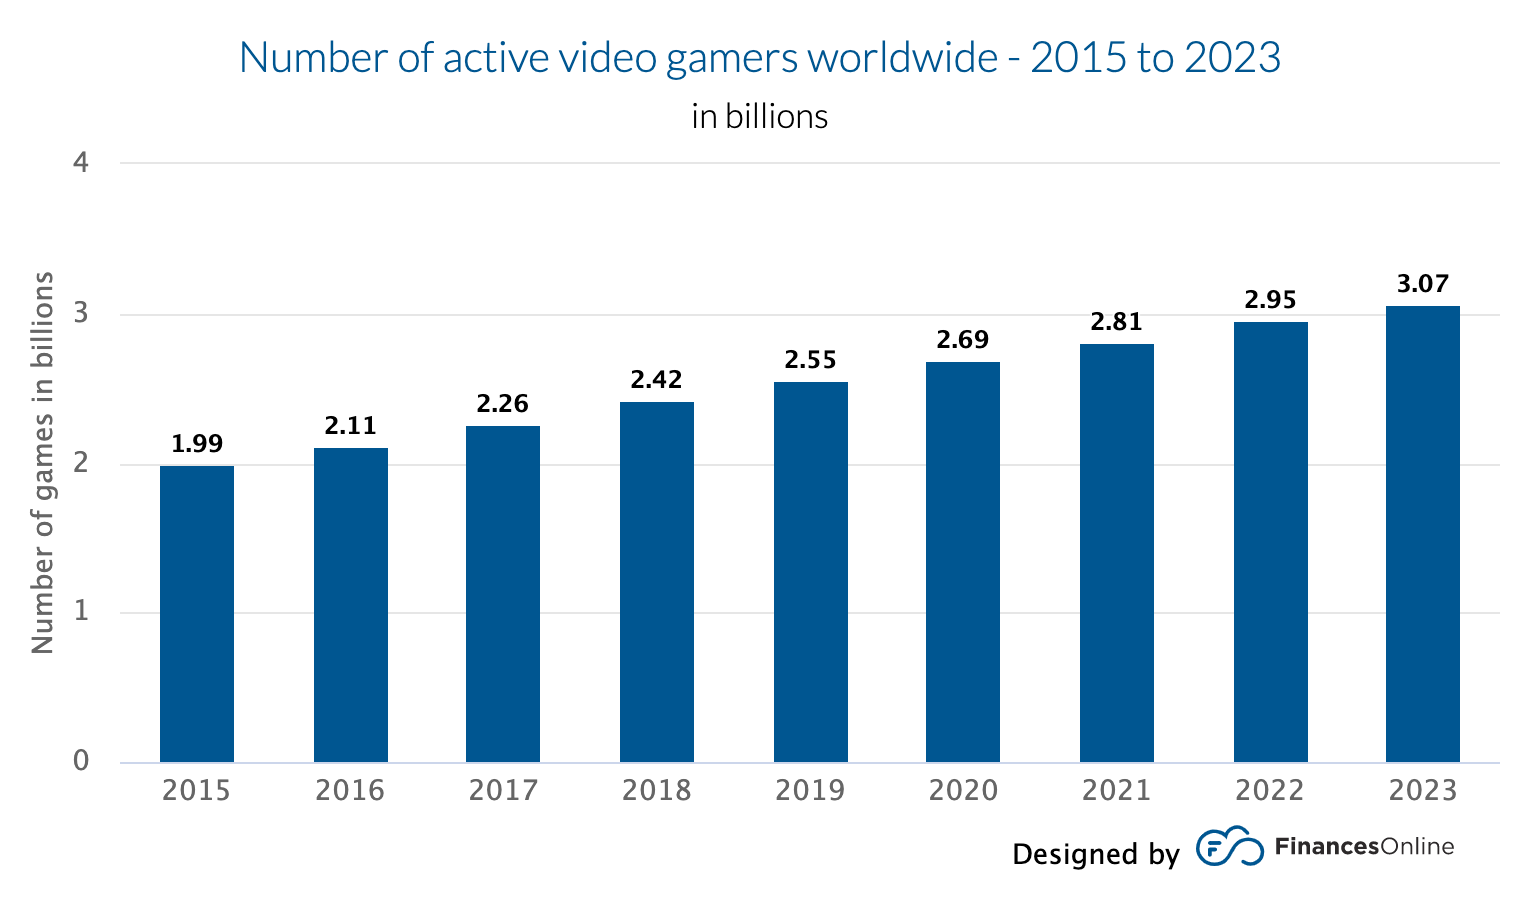
\includegraphics[width=8cm]{./assets/graph_active_gamers.png}}
\caption{Numbers of active gamers worldwide}\label{fig:model2}
\end{figure}

Looking further into the age group of gamers. Limelight's research(2020) suggests that every gamers ranging from age 18 - 64 years old spend at least 4.7 hours per week playing games, with the highest hours of 7.48 in 18 - 25 age group.

% Hours
\begin{figure}[!h]\centering
\setlength{\fboxrule}{0.2mm} % can define this in the preamble
\setlength{\fboxsep}{0.5mm}
\fbox{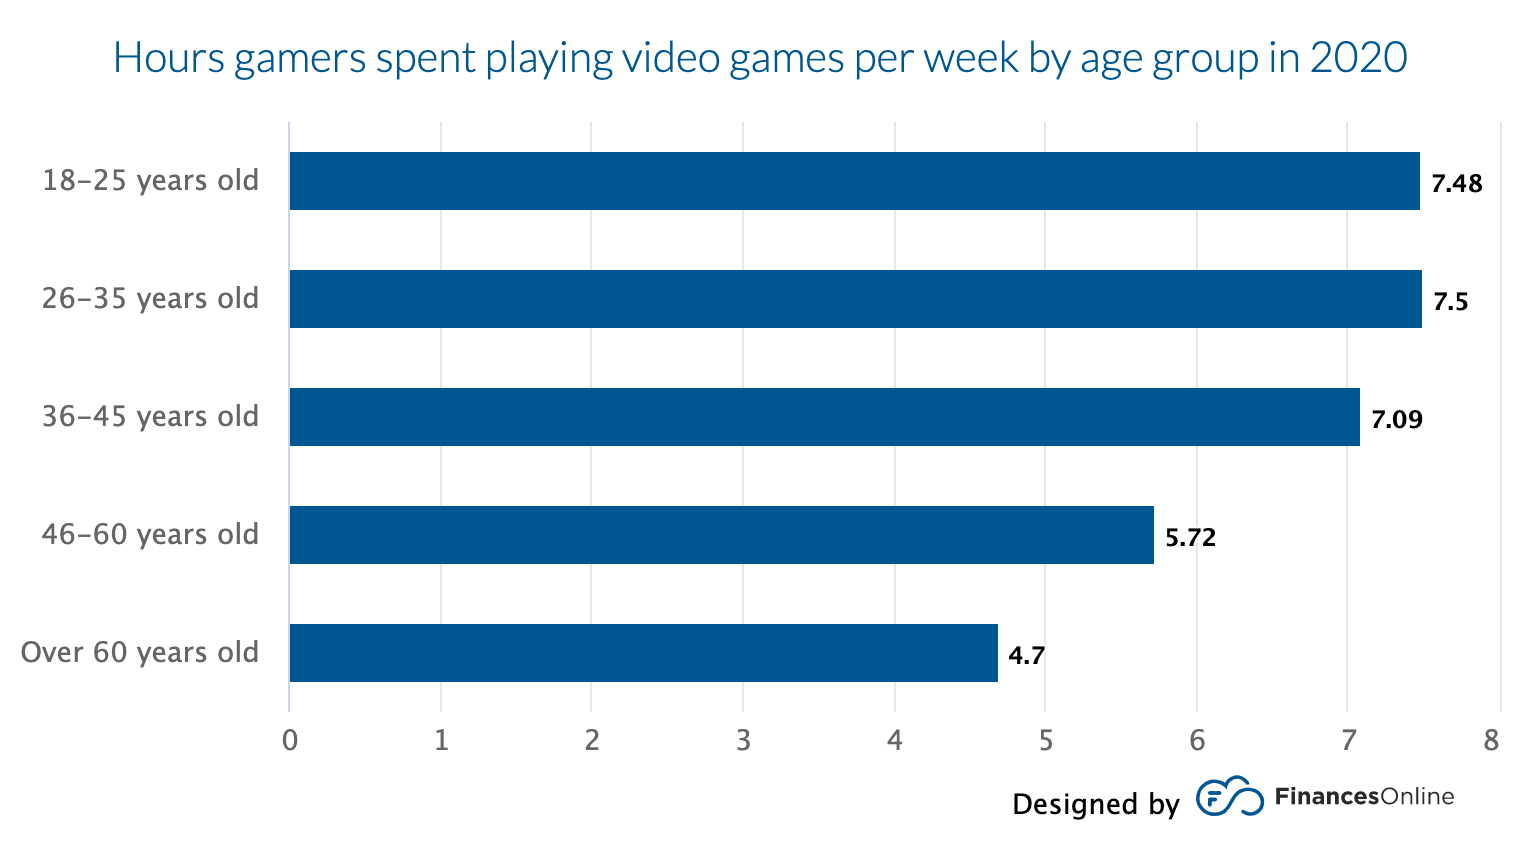
\includegraphics[width=8cm]{./assets/graph_gaming_hours.png}}
\caption{Average gaming hours per week by age group}\label{fig:model2}
\end{figure}

Game is currently one of the largest markets. Its revenues for 2020 reached over 159.3 billion US Dollars with almost half of market earnings generated by the Asia Pacific region. Evidently, game is a useful tool that can reach out to a broad range of people, which is why the demand for educational games are increasing especially during the pandemic where classes are taught online.\\[2cm]


\subsection{Application of Educational Games and its effectiveness}
\url{https://research.com/education/interactive-learning-statistics#5} provides statistics, demographics, and predictions related to educational games and active learning methods. [Imed Bouchrika]
Interactive learning is a learning method that supports the communications and interactions between educators and students. One of the effective ways to achieve active learning is through games. Juraschka (2019) showed that 74\% of teachers used game-based learning to enhance their lessons. This also applies in other settings other than the classroom as well, such as workplace and companies, which evidently increased the compound annual growth rate by half according to Ibáñez research (2018)\\

These research paper suggests the effects that educational games have on students.\\
\url{https://www.frontiersin.org/articles/10.3389/feduc.2021.623793/full} focused on educational games and learning effectiveness on college students [Siu Yin Cheung, Kai Yin Ng]\\
\url{https://www.sciencedirect.com/science/article/pii/S1875389212015933} analyzes the relationship between educational games and mathematics and logic. [Jing Li, Sujuan Ma, Linqing Ma]\\
\url{https://educationaltechnologyjournal.springeropen.com/articles/10.1186/s41239-017-0062-1} explores the effects of games and simulations on higher educatio.n [Dimitrios Vlachopoulos, Agoritsa Makri]\\
\url{https://www.researchgate.net/publication/233279860_Motivating_Children_to_Learn_Effectively_Exploring_the_Value_of_Intrinsic_Integration_in_Educational_Games}
suggests that motivations are the important aspect of using games as a educational tool. [Jacob Habgood, Shaaron Ainsworth]\\

Evidently, games are one of the effective methods to conduct interactive class and active learning for students. It can provide motivation and stimuli for students, and can effectively help them understand the concept they're trying to learn more deeply and entertainingly.


\subsection{Educational Game Specifications}
\url{https://www.researchgate.net/publication/267034149_Educational_Games_for_Teaching_Computer_Programming} page 3, in the topic educational games requirement specification suggests what aspects should be included in an effective educational game.\\
It is suggested that it should include two main aspects which are\\
1. Cognitive axis: Information intended to be received by the students should begin from the first category in the Bloom's taxonomy. 
\vspace{-5mm}
\paragraph{Bloom's Taxonomy} 

%------------------------------------------
\begin{wrapfigure}{lh}{7.5cm}
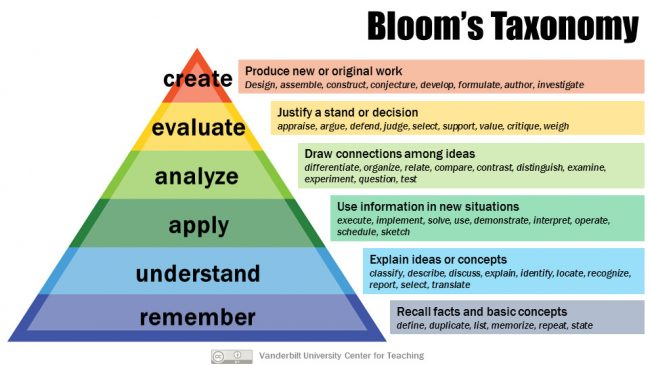
\includegraphics[width=7.5cm]{./assets/bloom.jpeg}
\end{wrapfigure} 
This is the structure of Bloom's Taxonomy, a taxonomy for teaching, learning, and assessment. It'll help us plan and design effective questions and puzzle for our game. Besides, we can ensure that our game lessons align with the objectives of teaching the fundamental of AI.
\\
\par
2. Emotional axis: Enable students to handle given situations through emotions, and using it to motivate students to solve and learn faster. So, they can experience the accomplishments when they get to the end of the story.